\section{eo\-Select\-One$<$ EOT, Worth\-T $>$ Class Template Reference}
\label{classeo_select_one}\index{eoSelectOne@{eoSelectOne}}
eo\-Select\-One selects only one element from a whole population.  


{\tt \#include $<$eo\-Select\-One.h$>$}

Inheritance diagram for eo\-Select\-One$<$ EOT, Worth\-T $>$::\begin{figure}[H]
\begin{center}
\leavevmode
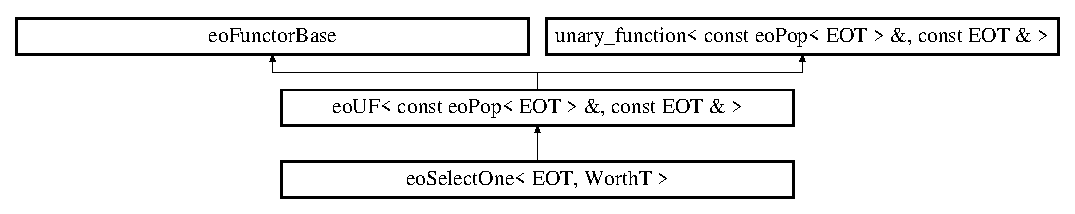
\includegraphics[height=2.42775cm]{classeo_select_one}
\end{center}
\end{figure}
\subsection*{Public Member Functions}
\begin{CompactItemize}
\item 
virtual void {\bf setup} (const {\bf eo\-Pop}$<$ {\bf EOT} $>$ \&\_\-pop)\label{classeo_select_one_a0}

\begin{CompactList}\small\item\em virtual function to setup some population stats (for instance eo\-Proportional can benefit greatly from this) \item\end{CompactList}\end{CompactItemize}


\subsection{Detailed Description}
\subsubsection*{template$<$class EOT, class Worth\-T = typename EOT::Fitness$>$ class eo\-Select\-One$<$ EOT, Worth\-T $>$}

eo\-Select\-One selects only one element from a whole population. 

Most selection techniques are simply repeated applications of eo\-Select\-One.

\begin{Desc}
\item[See also:]{\bf eo\-Select\-Many}{\rm (p.\,\pageref{classeo_select_many})}, eo\-Select\-Random, eo\-Det\-Tournament, eo\-Stoch\-Tournament, eo\-Proportional \end{Desc}




Definition at line 45 of file eo\-Select\-One.h.

The documentation for this class was generated from the following file:\begin{CompactItemize}
\item 
eo\-Select\-One.h\end{CompactItemize}
